O roteiro de dimensionamento para uma estrutura de solo reforçado é muito semelhante ao de uma estrutura não reforçada, com algumas análises diferenciadas devido à presença do reforço e a iteração do reforço com o solo.

Os principais manuais para o dimensionamento de estruturas de solo reforçado são: Federal Highway Administration. American Association of State Highway and Transportation Officials (FHWA, 2002);  \cite{aashto}; e o National Concrete Mansory Association (NCMA, 1997).


São realizadas as seguintes análises para os modos de ruptura:

\begin{itemize}
    \item Estabilidade Externa - Deslizamento, tombamento, capacidade de carga da fundação, e estabilidade global;
    \item Estabilidade Interna - Ruptura do reforço, arrancamento do reforço e conexão do reforço com a face.
\end{itemize}

\section{Estabilidade Externa}

Na análise da estabilidade externa considera-se que a massa de solo reforçado é similar a um muro de gravidade, e deve ser verificada a possibilidade de ocorrer quatro mecanismos clássicos de instabilidade em estruturas de contenção: deslizamento, tombamento, problema de capacidade de carga da fundação e ruptura global (Figura \ref{fig:estabilidade-externa}.

\begin{figure}[htb]
 \caption{Tipos de análise na verificação da estabilidade externa}
 \label{fig:estabilidade-externa}
 \centering
 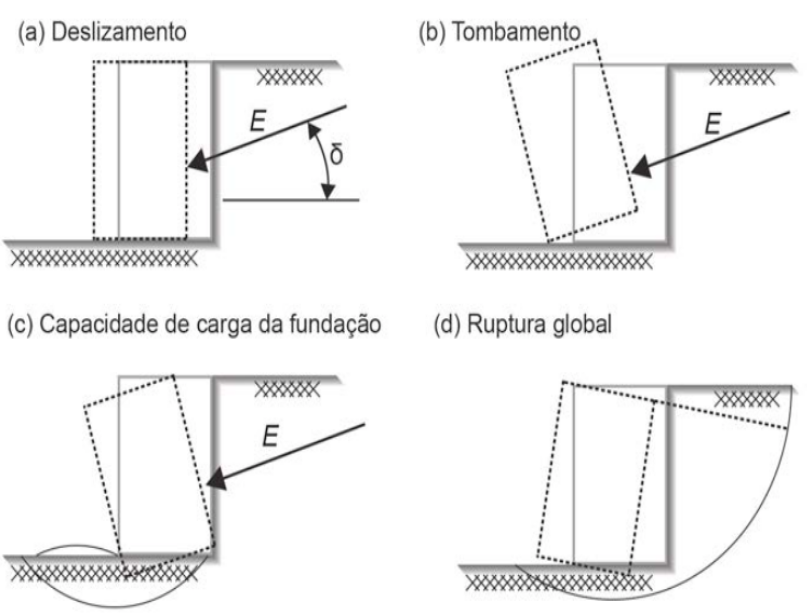
\includegraphics[scale=0.65]{estabilidade-externa.PNG}
 \fdireta{manual-geossinteticos}
\end{figure}

Para a determinação dos empuxos de solo $E$ que a massa de solo não reforçada exerce na massa de reforçada é possível adotar as teorias clássicas de equilíbrio limite. Para os cálculos será utilizada a formulação de Rankine, em que empuxos ativos são admitidos como sendo paralelos à superfície do terreno.

Devem ser consideradas as propriedades de curto e de longo prazos do solo, para verificação das condições durante a construção, durante a vida de serviço da estrutura e também em relação às mudanças que possam ocorrer de pressão neutra. O empuxo passivo atuante no pé do muro ou da estrutura de contenção abaixo do nível do terreno deve ser desprezado, na consideração das forças estabilizantes.

\subsection{Deslizamento}

A verificação da estabilidade ao escorregamento ou deslizamento da estrutura reforçada ao longo da sua base, na interface entre o aterro reforçado e o terreno de apoio, deve ser realizada usando as propriedades do solo reforçado ou do solo de apoio, aquele que for mais desfavorável. O fator de segurança ($FS_d$) utilizado é \textbf{1,5} para obras permanentes.

\begin{equation}
    FS_d = \frac{(\gamma_1 . H + q) . L_d . \tan(\phi)}{E_A} \geq 1,5
\end{equation}

Em que,

$FS_d$: fator de segurança ao deslizamento ao longo da base da estrutura;

$L_d$: comprimento do reforço ou largura da base da estrutura de solo reforçado;

$q$: sobrecarga uniformemente distribuída sobre o terrapleno;

$\gamma_1$: peso específico do solo 1;

$H$: altura da estrutura reforçada;

$\phi$: ângulo de atrito do solo de fundação ou solo do aterro, o que for menor;

$E$: Empuxo ativo calculado por Rankine.


\subsection{Tombamento}

Na verificação da segurança ao tombamento, o fator de segurança é calculado pela razão entre o momento resistente, devido ao peso da estrutura reforçada, e o momento atuante, exercido pelo empuxo de solo $E$. O fator de segurança ($FS_d$) recomendado neste caso é \textbf{2,0}.
 
 \begin{equation}
    FS_t = \frac{(\gamma_1 . H + q) . L_t}{2 . E . y_E} \geq 2,0
 \end{equation}
 
Em que,

$FS_t$: fator de segurança ao tombamento;

$L_t$: largura da estrutura reforçada ou comprimento do reforço;

$\gamma_E$: braço do momento do empuxo ativo, em relação ao pé da estrutura reforçada.
 
 \subsection{Capacidade de Carga da Fundação}
 
 A capacidade de carga máxima $q_{m\Acute{a}x}$ do solo de fundação pode ser avaliada pela equação de \citeonline{terzaghi:article} para uma fundação corrida.
 
 \begin{equation}
    q_{m\Acute{a}x} = c' . N_c + q_S . N_q = 0,5 . \gamma . B' . N_\gamma
 \end{equation}
 
 O fator de segurança para esta verificação é 3,0.
 
 \begin{equation}
 FS_t = \frac{q_{m\Acute{a}x}}{q_r} \geq 3,0
 \end{equation}
 
 Em que,
 
 $q_{m\Acute{a}x}$: capacidade de carga máxima do solo de fundação;
 
 $c'$: coesão do solo de fundação;
 
 $q_s$: sobrecarga ou nível da base da estrutura, caso esteja parcialmente enterrada;
 
 $\gamma$: peso específico do solo de fundação;
 
 $N_c, N_q, N_\gamma$: fatores de capacidade de carga;
 
 $q_r$: fator de capacidade de carga atuante na base do muro ou da estrutura;
 
 $R_v$: resultante das cargas verticais atuantes;
 
 $L$: comprimento do reforço na base do muro ou da estrutura;
 
 $e$: excentricidade da carga resultante $R_v$ em relação a linha central da base de largura $L$.
 
 
\subsection{Estabilidade Global}
 
Na verificação da estabilidade global é realizada a análise da estabilidade do maciço que contém a estrutura de solo reforçado, considerando que esta pode se deslocar como um corpo rígido no interior do maciço. Calcula-se o fator de segurança contra a rotação do maciço considerado, ao longo de uma superfície.

O fator de segurança recomendado é 1,5 e é obtido da seguinte forma:

\begin{equation}
    FS_g = \frac{\sum M_R}{\sum M_A}
\end{equation}

Em que:

$\sum M_R$: somatória dos momentos dos esforços resistentes em relação ao centro de rotação;

$\sum M_A$: somatória dos momentos dos esforços atuantes em relação ao centro de rotação.
 
 
\section{Estabilidade Interna}
 
O método recomendado para as análises da estabilidade interna é o proposto por \citeonline{mitchell:article}. Esse método é de simples aplicação e gera um dimensionamento verificado como adequado na prática.

É importante ressaltar que, por ser uma metodologia de países temperados, inicialmente o método não contempla o uso da coesão efetiva do nos cálculos. Contudo, a consideração desse parâmetro é de simples inserção no método, devendo ser incluído na determinação da força horizontal em cada camada do reforço e na resistência ao arrancamento do mesmo.
 
 Para evitar a ruptura dos reforços, o valor da tensão máxima atuante $T_m\Acute{a}x$ não deverá ser superior ao menor valor esperado para a resistência de projeto do geossintético $T_d$, amparado por um fator de segurança.
 
 A análise da estabilidade interna requer o conhecimento ou a adoção de valores do coeficiente do empuxo horizontal dentro da massa de solo reforçado. Projetistas que não possuem uma grande base de dados de estruturas reforçadas instrumentadas têm adotado o coeficiente de empuxo ativo, constante em toda a altura da estrutura, para a determinação das pressões horizontais.
 
 \subsection{Ruptura do Reforço}
 
 O sistema de reforços deve ser capaz de suportar as pressões transferidas pelo solo, sem romper. A pressão horizontal $\sigma_h$ em qualquer ponto da altura da estrutura pode ser determinada como: 
 
 \begin{equation}
     \sigma_h = k . \sigma_v
 \end{equation}
 Em que: 
 
 $k$: coeficiente de empuxo;
 
 $\sigma_v$: pressão vertical em qualquer profundidade
 
 
 
 \subsection{Arrancamento do Reforço}
 
A resistência ao arrancamento é desenvolvida por dois mecanismos de transferência de tensão, como ilustrado na Figura \ref{fig:transferencia-tensao}: 

\begin{enumerate}
    \item Atrito na superfície plana do reforço;
    \item Resistência passiva na superfície do reforço normal na direção do movimento relativo entre o solo e o reforço.
\end{enumerate}

\begin{figure}[htb]
 \caption{Mecanismos de transferência de tensão entre o solo e a geogrelha}
 \label{fig:transferencia-tensao}
 \centering
 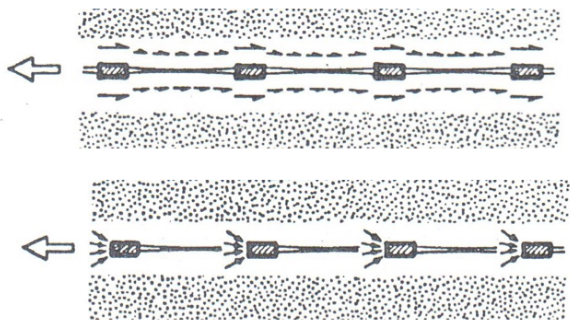
\includegraphics[scale=0.65]{transferencia-tensao.PNG}
 \fdireta{jewell:article}
\end{figure}
 
 
 


